% Appendix: calibrated evidence, sequential decisions, overlap, training-window length.
% Numbers are macros from tables/numbers_conf.tex (tools/unified/confidence_appendix.py).
\section{CONFIDENCE AND SEQUENTIAL DECISIONS}\label{app:conf}
Everything so far scores fixed windows. Here we ask how the decoder's per-window scores should
be combined over time, when a decision should be made, and whether overlapping windows or a
different training window help. Nothing in this appendix retrains the paper's models except
Sec.~\ref{app:conf:trainlen}; the decision rules only read their per-window scores.

\subsection{Theory}\label{app:conf:theory}
\textbf{Setting and notation.} A test trial is cut into consecutive, non-overlapping
windows $i=1,2,\dots$ of length $w$ seconds. Window $i$ has the recording $x_i$ and the two
candidate envelopes $a_{1,i},a_{2,i}$; we write $a_{\cdot,i}=(a_{1,i},a_{2,i})$,
$x_{1:n}=(x_1,\dots,x_n)$ and $a_{1:n}=(a_{\cdot,1},\dots,a_{\cdot,n})$. The attended index
$y\in\{1,2\}$ is fixed within the trial. $P_k$ and $\mathbb E_k$ denote probability and
expectation given $y=k$ (and the candidates), $\log$ is the natural logarithm,
$\Lambda$ is the logistic function, $\Lambda(\cdot)=1/(1+\exp(-\,\cdot\,))$, and $\Phi$ and $\varphi$ are the standard
normal distribution and density functions. The per-window log-likelihood ratio is
\[\ell_i=\log p(x_i\mid y{=}1,a_{\cdot,i})-\log p(x_i\mid y{=}2,a_{\cdot,i});\]
under the assumptions of Prop.~\ref{prop:pmi} it equals $\PMI(a_{1,i};x_i)-\PMI(a_{2,i};x_i)$.
After $n$ windows the accumulated evidence is $S_n=\sum_{i=1}^n\ell_i$ ($S_0=0$). A real
statistic $\hat\ell$ is \emph{calibrated} when $P(y{=}1\mid\hat\ell)=\Lambda(\hat\ell)$. A decoder gives the
candidates scores $s_{1,i},s_{2,i}$ (Sec.~\ref{sec:theory}); we calibrate their margin
$\Delta s_i=s_{1,i}-s_{2,i}$ by one scale, $\hat\ell_i=\beta\,\Delta s_i$, with $\beta>0$ fitted by the
logistic loss on the fold's validation windows, and use $\hat\ell_i$ in place of $\ell_i$. A
positive scale never changes a single-window decision; it matters only when windows are
combined.

\begin{proposition}[additive evidence]\label{prop:add}
Assume (a) given $y$ and all candidates, the $x_i$ are independent and $x_i$ depends on the
candidates only through $a_{y,i}$; (b) $P(y{=}1)=\tfrac12$ independently of the candidates.
Then $\log\frac{P(y=1\mid x_{1:n},a_{1:n})}{P(y=2\mid x_{1:n},a_{1:n})}=S_n$, i.e.\ $S_n$ is
calibrated, and the decision with the fewest errors given $n$ windows is $\mathrm{sign}\,S_n$. Majority
voting over $\mathrm{sign}\,\ell_i$ is optimal only when all $|\ell_i|$ are equal.
\end{proposition}

\begin{proposition}[accumulation law as an information rate]\label{prop:gauss}
Let the $\ell_i$ of Prop.~\ref{prop:add} be independent and identically distributed
(i.i.d.)\ given $y$, with
$\ell_i\mid y{=}1\sim\mathcal N(\mu,\nu^2)$ for some $\mu>0$, $\nu^2>0$. Then (i)
$\nu^2=2\mu$ and $\ell_i\mid y{=}2\sim\mathcal N(-\mu,2\mu)$; (ii) $\mu$ is the
Kullback--Leibler divergence $D_{\mathrm{KL}}\big(p(x_i\mid y{=}1)\,\|\,p(x_i\mid y{=}2)\big)$,
the information one window carries about $y$; (iii) with the information rate $\mathcal I=\mu/w$ (nats
per second) and a fixed decision length of $T=nw$ seconds ($n$ windows),
\[P(\mathrm{correct}\mid T)=\Phi\big(\sqrt{\mathcal I T/2}\big)=\Phi(\kappa\sqrt T),\qquad
\kappa^2=\mathcal I/2 .\]
\end{proposition}
Prop.~\ref{prop:gauss} gives Prop.~\ref{prop:law} a decision-theoretic reading that does not
rely on the decoder being a correlation: $2\kappa^2$ is the information the brain response
carries about the attended talker, per second. It also gives a check of calibration and of
the Gaussian model: by (i), exact Gaussian log-likelihood ratios have
$\mathrm{Var}_1(\ell_i)/(2\,\mathbb E_1\ell_i)=1$, where $\mathrm{Var}_1$ is the variance
under $P_1$; we evaluate it on test windows with the log-odds oriented so that the attended
candidate is candidate 1.

\begin{proposition}[voting wastes evidence]\label{prop:vote}
Under Prop.~\ref{prop:gauss} let $q=\Phi(\sqrt{\mu/2})$ be the one-window accuracy. Summing
$n$ windows gives $\Phi(\sqrt n\,\Phi^{-1}(q))$. Majority voting gives, for large $n$,
$\Phi\big(\sqrt n\,(2q-1)/(2\sqrt{q(1-q)})\big)$. As $\mu\to0$ voting needs
$\pi/2\approx1.57$ times as many windows as summing for the same accuracy.
\end{proposition}

\begin{proposition}[sequential decisions]\label{prop:sprt}
Under Prop.~\ref{prop:gauss}, fix a threshold $A>0$ and let
$N=\min\{n:|S_n|\ge A\}$ be the number of windows the rule reads before
$|S_n|$ first reaches $A$; the rule decides $\mathrm{sign}\,S_N$ after $T_A=Nw$ seconds
(Wald's sequential probability ratio test with symmetric thresholds). Neglecting the overshoot
of $S_N$ beyond $\pm A$, (i) its error rate is $\alpha=1/(1+e^{A})$; (ii) its mean decision
time is
\[\mathbb E[T_A]=\frac{(1-2\alpha)\,\log\frac{1-\alpha}{\alpha}}{2\kappa^2}\ \text{s};\]
(iii) no rule with both error rates $\le\alpha$ has a smaller mean decision time under
either hypothesis \citep{wald1948optimum}. A fixed-length decision reaches the same error rate
$\alpha$ after $T_{\rm fix}=(\Phi^{-1}(1-\alpha)/\kappa)^2$ seconds (Prop.~\ref{prop:gauss}),
so $\mathbb E[T_A]/T_{\rm fix}=0.59,\,0.54,\,0.49,\,0.42$ at $\alpha=0.2,\,0.1,\,0.05,\,0.01$,
decreasing to $1/4$ as $\alpha\to0$.
\end{proposition}
The sequential rule reaches the fixed-window accuracy in about half the time, with the
same $\kappa$. This is the classical result of \citet{wald1945sequential}; its continuous-time
limit is the drift--diffusion model of perceptual decisions \citep{bogacz2006physics}. It
rests on two assumptions that EEG violates to some degree, independence of consecutive
windows and a constant information rate; we measure both below. If the information rate varies
between stretches of a trial (attention lapses, noise bursts), the sequential rule spends its
time on the weak stretches, which a fixed window cannot do.

\begin{proposition}[stopping does not bias the posterior]\label{prop:stop}
Under the assumptions of Prop.~\ref{prop:add}, let $N$ be any stopping time of the window
sequence, i.e.\ whether to stop after window $n$ depends only on $x_{1:n}$ and $a_{1:n}$, and
decide $\mathrm{sign}\,S_N$. Then $P(\text{correct}\mid x_{1:N})=\Lambda(|S_N|)$. In particular
every decision taken when $|S_N|\ge A$ is correct with probability at least $\Lambda(A)$,
\emph{whatever its length}, and the accuracy of the sequential rule is set by the threshold
alone; the length only adapts to how fast the evidence arrives.
\end{proposition}

\begin{proposition}[overlapping windows]\label{prop:overlap}
Let the evidence be additive in time: the log-likelihood ratio of the data in
$[t_0,t_1)$ is $\ell(t_0,t_1)=\int_{t_0}^{t_1}\dot\ell(t)\,dt$ for a log-likelihood-ratio density
$\dot\ell(t)$ (nats per second). Let windows of length $w$ start at $t_j=jh$, $j=0,1,\dots$,
every $h=w/J$ seconds for an integer $J\ge1$ ($J=1$: no overlap). Over a stretch of length $T\gg w$, the sum of the
overlapping windows' log-odds equals $J$ times the log-odds of the stretch, up to edge terms
of length $<w$. Hence (i) the sign, and so a fixed-length decision, is unchanged: overlap adds
no information; (ii) the summed log-odds overstate the evidence by the factor $J$ and must be
multiplied by $h/w$ to stay calibrated; (iii) with that correction the sequential rule is the
one of Prop.~\ref{prop:sprt} checked every $h$ instead of every $w$ seconds, which only
reduces the overshoot.
\end{proposition}

\paragraph{Proofs.}
\emph{Prop.~\ref{prop:add}.} By Bayes' rule and (b), the posterior ratio equals the likelihood
ratio $p(x_{1:n}\mid y{=}1,a_{1:n})/p(x_{1:n}\mid y{=}2,a_{1:n})$. By (a) each likelihood
factorises over windows into $\prod_i p(x_i\mid y,a_{\cdot,i})$, so the logarithm of the ratio
is $\sum_i\ell_i=S_n$; hence $P(y{=}1\mid x_{1:n},a_{1:n})=\Lambda(S_n)$. The minimum-error
decision picks the larger posterior, i.e.\ $\mathrm{sign}\,S_n$. The majority vote depends on
the signs of the $\ell_i$ only; it agrees with $\mathrm{sign}\,S_n$ for every configuration of
signs only if all $|\ell_i|$ are equal. \qed

\emph{Prop.~\ref{prop:gauss}.} Let $p_1,p_2$ be the densities of $\ell_i$ under $P_1,P_2$.
Since $\ell_i$ is the log-likelihood ratio of $x_i$, the change of measure from $P_1$ to $P_2$
multiplies densities by $e^{-\ell_i}$, so $p_2(\ell)=e^{-\ell}p_1(\ell)$. With
$p_1=\mathcal N(\mu,\nu^2)$, $p_2$ integrates to one only if
$\mathbb E_1 e^{-\ell_i}=e^{-\mu+\nu^2/2}=1$, i.e.\ $\nu^2=2\mu$; completing the square then
gives $p_2=\mathcal N(\mu-\nu^2,\nu^2)=\mathcal N(-\mu,2\mu)$, which is (i). (ii) holds by
definition, $D_{\mathrm{KL}}=\mathbb E_1\log\frac{p(x_i\mid y=1)}{p(x_i\mid y=2)}
=\mathbb E_1\ell_i=\mu$. For (iii), independence gives $S_n\mid y{=}1\sim\mathcal N(n\mu,2n\mu)$,
so $P_1(S_n>0)=\Phi(n\mu/\sqrt{2n\mu})=\Phi(\sqrt{n\mu/2})$; by (i) the same holds for
$P_2(S_n<0)$. Substituting $n\mu=\mathcal I T$ and $\kappa^2=\mathcal I/2$ gives the claim. \qed

\emph{Prop.~\ref{prop:vote}.} Summing: by Prop.~\ref{prop:gauss}(iii) the accuracy is
$\Phi(\sqrt{n\mu/2})$, and $\sqrt{\mu/2}=\Phi^{-1}(q)$ by the definition of $q$. Voting: the
number of correctly signed windows is binomial with parameters $n$ and $q$; by the central limit
theorem the majority is right with probability
$\Phi\big((nq-n/2)/\sqrt{nq(1-q)}\big)=\Phi\big(\sqrt n\,(2q-1)/(2\sqrt{q(1-q)})\big)$. For small
$\mu$, $q-\tfrac12\approx\varphi(0)\sqrt{\mu/2}$ with $\varphi(0)=1/\sqrt{2\pi}$, and
$q(1-q)\approx\tfrac14$, so the argument of $\Phi$ is $\sqrt n\,\sqrt{2/\pi}\,\sqrt{\mu/2}$ for
voting against $\sqrt n\,\sqrt{\mu/2}$ for summing; equal accuracy needs
$n_{\rm vote}/n_{\rm sum}=\pi/2$ windows (the asymptotic relative efficiency of the sign test).
\qed

\emph{Prop.~\ref{prop:sprt}.} $N$ is finite with probability one because $S_n$ drifts to
$\pm\infty$. (i) Changing measure as in the proof of Prop.~\ref{prop:gauss}, the probability of
a wrong decision under $y{=}2$ is $P_2(S_N\ge A)=\mathbb E_1[e^{-S_N};\,S_N\ge A]$. Without
overshoot $S_N\in\{-A,A\}$, so this equals $e^{-A}P_1(S_N\ge A)=e^{-A}(1-\alpha)$, where
$\alpha$ is the error rate; by the symmetry of (i) in Prop.~\ref{prop:gauss} the error rate is
the same under both hypotheses, so $\alpha=e^{-A}(1-\alpha)$, i.e.\ $\alpha=1/(1+e^A)$ and
$A=\log\frac{1-\alpha}{\alpha}$. (ii) Wald's identity gives $\mathbb E_1S_N=\mu\,\mathbb E_1N$,
and without overshoot $\mathbb E_1S_N=A(1-\alpha)-A\alpha$, so
$\mathbb E_1N=A(1-2\alpha)/\mu$ windows (the same under $P_2$). Then
$\mathbb E[T_A]=w\,\mathbb E N=A(1-2\alpha)\,w/\mu$, and $\mu=\mathcal I w=2\kappa^2w$ by
Prop.~\ref{prop:gauss} gives the stated time. (iii) is the Wald--Wolfowitz theorem for i.i.d.\
increments. $T_{\rm fix}$ solves $\Phi(\kappa\sqrt{T})=1-\alpha$, and the ratio follows by
division. As $\alpha\to0$, $\log\frac{1-\alpha}{\alpha}\sim\log\frac1\alpha$ and
$\Phi^{-1}(1-\alpha)^2\sim2\log\frac1\alpha$, so the ratio tends to $1/4$. With overshoot,
$|S_N|>A$: the realised error rate is below $1/(1+e^A)$ and the time above (ii), both by at
most one window's increment. \qed

\emph{Prop.~\ref{prop:stop}.} Because $N$ is a stopping time, the event $\{N=n\}$ is
determined by $(x_{1:n},a_{1:n})$, so conditioning on it adds nothing to them:
$P(y{=}1\mid x_{1:N},a_{1:N},N{=}n)=P(y{=}1\mid x_{1:n},a_{1:n})=\Lambda(S_n)$ by
Prop.~\ref{prop:add}. The decision $\mathrm{sign}\,S_N$ is therefore correct with probability
$\Lambda(|S_N|)$, which is at least $\Lambda(A)$ whenever $|S_N|\ge A$. This is the likelihood
principle: the posterior does not depend on the stopping rule. \qed

\emph{Prop.~\ref{prop:overlap}.} Consider the stretch $[0,T)$ and let $\chi(t)$ be the number of
windows $[t_j,t_j+w)$ inside it that contain the time $t$. Every $t$ at distance at least $w$
from both ends of the stretch lies in exactly $J=w/h$ windows, so $\chi(t)=J$ there, and
$\chi(t)<J$ only within $w$ of the ends. Summing the window log-odds,
$\sum_j\ell(t_j,t_j+w)=\int_0^T\dot\ell(t)\,\chi(t)\,dt=J\,\ell(0,T)+E$, where the edge term $E$
involves only data within $w$ of the ends. Hence the sum has the sign of the stretch's
log-likelihood ratio $\ell(0,T)$ up to $E$ (i), and it is $J$ times the calibrated value (ii).
Multiplied by $1/J=h/w$, the running sum after each new window equals the log-likelihood ratio
of the data read so far, up to the edge term; this is the statistic $S$ of
Prop.~\ref{prop:sprt} evaluated every $h$ instead of every $w$ seconds (iii). \qed

\paragraph{Related rules.} \citet{geirnaert2020interpretable} turn fixed-window accuracies
into the minimal expected switch duration of a gain-control Markov chain; the sequential rule
can feed that chain the same way. Bayesian state-space filtering \citep{miran2018realtime}
additionally models attention switches, which our datasets do not contain. Calibration by one
scale is temperature scaling \citep{guo2017calibration}; averaging the calibrated log-odds of
independently trained models is a deep ensemble \citep{lakshminarayanan2017simple}.

\subsection{Calibration and combining windows}\label{app:conf:calib}
Table~\ref{tab:conf_calib}. Raw margins are over-confident (expected calibration error, ECE, \confEceRawMin--\confEceRawMax{}
on the two-talker sets); one scale fitted on validation brings every dataset to
ECE $\le$\,\confEceCalMax. Averaging the calibrated log-odds of the three seeds adds
\confEnsMin--\confEnsMax{} points at 5\,s. Summing a trial's log-odds instead of majority voting changes accuracy by
\confSumMin{} to \confSumMax{} points (Prop.~\ref{prop:vote}). The calibrated 1-s log-odds have
$\mathrm{Var}/(2\,\mathrm{mean})=$\,\confVarMin--\confVarMax{} (exactly 1 for Gaussian
log-likelihood ratios) and lag-1 autocorrelation \confLagMin--\confLagMax: consecutive windows
are close to, but not exactly, independent.
\begin{table*}[h]\centering\small
\caption{Calibration and combination of windows (test folds; mean of 3 seeds unless marked).
ECE: expected calibration error, 10 bins; NLL: log-loss in bits (chance 1). ens.: average of
the 3 seeds' calibrated log-odds. Trial: one decision per trial by majority vote of the 5-s
windows or by the sign of their summed log-odds. Last two columns: diagnostics of
Prop.~\ref{prop:gauss} on the 1-s log-odds.}\label{tab:conf_calib}
\begin{tabular}{lcccccccccc}\toprule
& \multicolumn{2}{c}{ECE (5\,s)} & \multicolumn{2}{c}{NLL, bits (5\,s)} & \multicolumn{2}{c}{acc.\ 5\,s} & \multicolumn{2}{c}{trial} & \multicolumn{2}{c}{1-s log-odds} \\
Dataset & raw & cal. & raw & cal. & single & ens. & vote & sum & $\frac{\mathrm{var}}{2\,\mathrm{mean}}$ & lag-1 $r$ \\\midrule
KU Leuven & 0.113 & 0.022 & 0.91 & 0.78 & 72.7 & 74.3 & 97.6 & 99.3 & 1.11 & 0.05 \\
DTU & 0.111 & 0.012 & 0.86 & 0.70 & 76.2 & 78.3 & 94.6 & 97.0 & 1.04 & 0.05 \\
Fuglsang'20 & 0.078 & 0.016 & 0.72 & 0.64 & 79.6 & 81.2 & 96.8 & 98.5 & 0.99 & 0.05 \\
ESAA & 0.098 & 0.016 & 0.82 & 0.68 & 77.9 & 80.0 & 95.6 & 97.1 & 1.03 & 0.05 \\
KUL-255ch & 0.143 & 0.028 & 1.04 & 0.84 & 69.4 & 71.5 & 99.6 & 99.4 & 1.13 & 0.05 \\
Broderick & 0.171 & 0.019 & 1.13 & 0.90 & 63.6 & 65.7 & 78.9 & 83.1 & 1.03 & 0.05 \\
SparrKULee & 0.014 & 0.002 & 0.28 & 0.27 & 92.3 & 93.0 & -- & -- & 0.98 & 0.05 \\
MEG-MASC & 0.014 & 0.001 & 0.05 & 0.04 & 99.0 & 99.3 & -- & -- & 1.05 & 0.01 \\
\bottomrule\end{tabular}

\end{table*}

\subsection{Sequential decisions}\label{app:conf:seq}
Fig.~\ref{fig:conf_seq} and Table~\ref{tab:conf_seq} compare the sequential rule of
Prop.~\ref{prop:sprt} on calibrated 1-s log-odds with fixed-length decisions that sum the
same 1-s log-odds over $T$\,s, at equal mean decision time. Both rules see exactly the same
scores; only the stopping differs. Thresholds $A$ are fixed values, not tuned. For
CoupleFlow the sequential rule gains \confGainOneMin--\confGainOneMax{} points at $A{=}1$ and
\confGainTwoMin--\confGainTwoMax{} at $A{=}2$; for the linear backward model it gains
\confLinGainOneMin--\confLinGainOneMax{} and \confLinGainTwoMin--\confLinGainTwoMax. The gain
is therefore a property of the decision rule, available to any calibrated decoder; the
ranking of decoders is set by $\kappa$, which is larger for CoupleFlow on every dataset except
Broderick. The observed mean times are \confTheoryRatioMin--\confTheoryRatioMax{} times Wald's
prediction from the fitted $\kappa$ (dotted lines). Overshoot on the 1-s grid lengthens the
observed times; a varying information rate within trials shortens them, since the rule stops
early on strong stretches, which the i.i.d.\ prediction ignores.
``Time'' counts speech windows; every decision also needs the EEG of the neural lag
(up to 1.1\,s) after its last window, for fixed and sequential rules alike. Decision times are
spread: Table~\ref{tab:conf_seq} gives their 90th percentile next to the mean.
\begin{figure*}[h]\centering
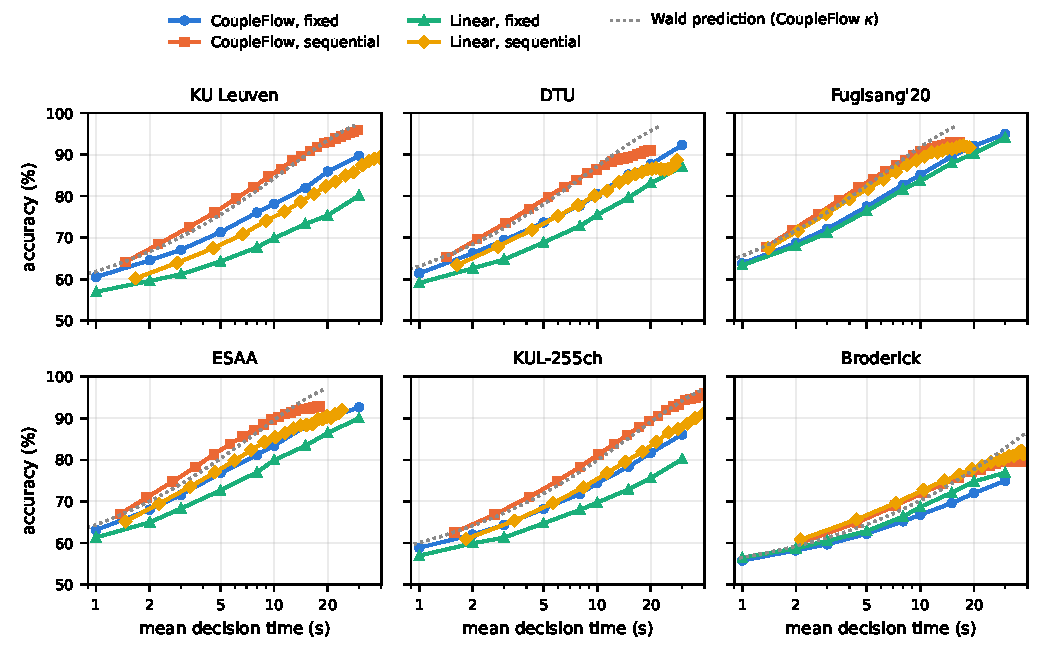
\includegraphics[width=0.9\textwidth]{figures/conf_seq.pdf}
\caption{Accuracy against mean decision time, two-talker datasets (test folds). Fixed:
sign of the summed calibrated log-odds of $T$ consecutive 1-s windows. Sequential: the rule
of Prop.~\ref{prop:sprt} at thresholds $A=0.25,\dots,5$. Dotted: Wald's prediction from
CoupleFlow's fitted $\kappa$ (Prop.~\ref{prop:sprt}). CoupleFlow: mean of 3 seeds.}
\label{fig:conf_seq}
\end{figure*}
\begin{table*}[h]\centering\small
\caption{Sequential against fixed-length decisions on calibrated 1-s log-odds. $\kappa$: fit
of $\Phi(\kappa\sqrt T)$ to the fixed-length curve. Cells: sequential accuracy (\%) / mean
decision time (s) (90th percentile) / fixed-length accuracy at the same mean time (\%). Gain: sequential minus
fixed at $A{=}2$ (points).}\label{tab:conf_seq}
\resizebox{\textwidth}{!}{\begin{tabular}{lcccccccc}\toprule
& \multicolumn{4}{c}{CoupleFlow (mean of 3 seeds)} & \multicolumn{4}{c}{Linear backward model} \\
\cmidrule(lr){2-5}\cmidrule(lr){6-9}
Dataset & $\kappa$ & $A{=}1$ & $A{=}2$ & gain & $\kappa$ & $A{=}1$ & $A{=}2$ & gain \\\midrule
KU Leuven & 0.240 & 76.0 / 4.6 (9) / 70.5 & 86.6 / 10.9 (22) / 78.8 & +7.7 & 0.158 & 70.8 / 6.7 (13) / 66.1 & 80.6 / 16.7 (34) / 74.0 & +6.6 \\
DTU & 0.267 & 77.0 / 4.1 (8) / 71.8 & 85.5 / 8.8 (17) / 78.8 & +6.7 & 0.213 & 75.2 / 6.0 (12) / 70.2 & 83.3 / 13.3 (27) / 78.2 & +5.1 \\
Fuglsang'20 & 0.318 & 79.1 / 3.5 (7) / 73.5 & 87.5 / 7.3 (14) / 81.5 & +6.0 & 0.299 & 79.2 / 4.0 (8) / 73.7 & 87.4 / 8.4 (16) / 82.0 & +5.4 \\
ESAA & 0.292 & 78.3 / 3.6 (7) / 73.2 & 87.3 / 7.7 (15) / 80.8 & +6.5 & 0.250 & 77.0 / 4.6 (9) / 71.9 & 85.4 / 10.1 (20) / 80.0 & +5.4 \\
KUL-255ch & 0.203 & 74.9 / 5.9 (12) / 69.4 & 86.0 / 14.7 (30) / 78.1 & +7.9 & 0.159 & 73.4 / 8.4 (17) / 68.3 & 84.3 / 21.5 (43) / 76.3 & +8.0 \\
Broderick & 0.131 & 72.1 / 10.4 (22) / 66.8 & 77.7 / 22.0 (50) / 72.4 & +5.3 & 0.146 & 72.8 / 10.4 (21) / 69.0 & 78.6 / 22.2 (46) / 75.3 & +3.3 \\
\bottomrule\end{tabular}
}
\end{table*}

\subsection{Anatomy of the sequential decisions}\label{app:conf:anatomy}
Table~\ref{tab:conf_seq_detail} and Figs.~\ref{fig:conf_threshold} and~\ref{fig:conf_len}
open up the sequential rule on CoupleFlow's calibrated 1-s log-odds (decisions of the three
seeds pooled, test folds). Four things stand out.

\emph{The threshold sets the accuracy.} Decisions that reach the threshold are about as
accurate as the guarantee $\Lambda(A)$ of Prop.~\ref{prop:stop}
(Fig.~\ref{fig:conf_threshold}a; deviation \confDetAboveMin{} to \confDetAboveMax{} points over
all datasets and thresholds). At small $A$ they are above it, because a 1-s step overshoots
the threshold; at large $A$ slightly below it, the signature of the mild positive dependence
between consecutive windows, which makes long sums a little over-confident. At $A{=}1$
decisions are \confDetOneAccMin--\confDetOneAccMax\% correct ($\Lambda(1)=$\,\confDetOneNominal\%),
at $A{=}2$ \confDetTwoAccMin--\confDetTwoAccMax\% ($\Lambda(2)=$\,\confDetTwoNominal\%), on every
dataset: a target accuracy fixes $A$, to within a few points, without looking at the data.

\emph{The chosen length adapts widely.} The same threshold yields short and long decisions
(Fig.~\ref{fig:conf_len}a). At $A{=}1$ the median decision uses
\confDetOneMedMin--\confDetOneMedMax\,s and the 90th percentile \confDetOnePNineMin--\confDetOnePNineMax\,s;
\confDetOneOneSec--\confDetOneOneSecMax\% of decisions are taken after a single second. At
$A{=}2$ the median is \confDetTwoMedMin--\confDetTwoMedMax\,s and the 90th percentile
\confDetTwoPNineMin--\confDetTwoPNineMax\,s. The mean length grows with $A$ roughly as
$A(1-2\alpha)/(2\kappa^2)$ (Prop.~\ref{prop:sprt}), so datasets with small $\kappa$ (Broderick,
KUL-255ch) wait longest (Fig.~\ref{fig:conf_threshold}b).

\emph{Accuracy hardly depends on the chosen length.} As Prop.~\ref{prop:stop} predicts, fast
and slow decisions are about equally accurate (Fig.~\ref{fig:conf_len}b): decisions of
at most 8\,s are at most \confDetShortDevMax{} points below $\Lambda(2)$. The exception is the
longest decisions ($\ge$17\,s), up to \confDetLongDevMax{} points below $\Lambda(2)$. They come
from stretches in which the recording tracks the speech poorly, and one global calibration
scale over-states the evidence of such windows: calibration holds on average, not
conditionally on the local signal quality. A calibration that depends on the recent evidence
rate would close this gap.

\emph{Finite trials force some decisions.} When a trial ends before $|S|$ reaches $A$, the
leftover is decided anyway (Fig.~\ref{fig:conf_threshold}c). These forced decisions are less
accurate (\confDetForcedAccMin--\confDetForcedAccMax\% at $A\in\{1,2\}$) and frequent on the
short trials of \confDetForcedWorst{} (up to \confDetTwoForcedMax\% at $A{=}2$); the ``all''
column includes them. In continuous listening there is no trial end and they do not arise.

\begin{table*}[h]\centering\small
\caption{Anatomy of the sequential rule (CoupleFlow, calibrated 1-s log-odds, 3 seeds
pooled, test folds). $\Lambda(A)$: accuracy guaranteed by Prop.~\ref{prop:stop} for decisions
that reach the threshold. Accuracy of all decisions and of those that reached the threshold
(decided). Chosen length: mean, median and 10th--90th percentile of the number of seconds a
decision used. Forced: share and accuracy of decisions cut by the end of a trial. Fixed:
fixed-length accuracy at the same mean length; gain in points.}\label{tab:conf_seq_detail}
\resizebox{\textwidth}{!}{\begin{tabular}{lccccccccccc}\toprule
& & \multicolumn{3}{c}{accuracy (\%)} & \multicolumn{3}{c}{chosen length (s)} & \multicolumn{2}{c}{forced at trial end} & \multicolumn{2}{c}{vs.\ fixed length} \\
\cmidrule(lr){3-5}\cmidrule(lr){6-8}\cmidrule(lr){9-10}\cmidrule(lr){11-12}
Dataset & $A$ & $\Lambda(A)$ & all & decided & mean & median & 10--90\% & share (\%) & acc.\ (\%) & fixed (\%) & gain \\\midrule
KU Leuven & 0.5 & 62.2 & 68.4 & 68.5 & 2.2 & 2 & 1--4 & 0.5 & 60.1 & 65.1 & +3.3 \\
 & 1 & 73.1 & 76.0 & 76.2 & 4.6 & 4 & 1--9 & 1.6 & 65.3 & 70.5 & +5.5 \\
 & 1.5 & 81.8 & 82.1 & 82.6 & 7.6 & 6 & 2--15 & 2.9 & 66.6 & 75.5 & +6.7 \\
 & 2 & 88.1 & 86.5 & 87.3 & 10.9 & 8 & 3--22 & 4.4 & 70.9 & 78.8 & +7.7 \\
 & 3 & 95.3 & 91.8 & 93.1 & 17.4 & 13 & 5--35 & 7.2 & 74.1 & 83.9 & +7.9 \\
 & 4 & 98.2 & 94.3 & 96.4 & 23.7 & 19 & 8--47 & 10.0 & 75.9 & 87.3 & +7.0 \\
\midrule
DTU & 0.5 & 62.2 & 69.6 & 70.0 & 2.1 & 2 & 1--4 & 2.4 & 55.5 & 66.6 & +3.0 \\
 & 1 & 73.1 & 77.0 & 78.2 & 4.1 & 3 & 1--8 & 6.9 & 60.5 & 71.8 & +5.1 \\
 & 1.5 & 81.8 & 82.2 & 84.4 & 6.5 & 5 & 2--13 & 12.1 & 66.4 & 75.7 & +6.6 \\
 & 2 & 88.1 & 85.5 & 88.9 & 8.8 & 7 & 3--18 & 17.3 & 69.3 & 78.8 & +6.7 \\
 & 3 & 95.3 & 88.8 & 94.5 & 13.1 & 11 & 4--26 & 26.5 & 72.9 & 83.3 & +5.4 \\
 & 4 & 98.2 & 90.2 & 97.0 & 16.8 & 14 & 6--33 & 34.8 & 77.4 & 86.0 & +4.1 \\
\midrule
Fuglsang'20 & 0.5 & 62.2 & 71.8 & 72.1 & 1.9 & 1 & 1--4 & 2.0 & 54.6 & 68.3 & +3.5 \\
 & 1 & 73.1 & 79.1 & 80.2 & 3.5 & 3 & 1--7 & 5.4 & 59.7 & 73.5 & +5.6 \\
 & 1.5 & 81.8 & 84.2 & 86.3 & 5.4 & 4 & 2--11 & 9.3 & 63.8 & 78.2 & +6.0 \\
 & 2 & 88.1 & 87.5 & 90.6 & 7.3 & 6 & 2--14 & 13.4 & 67.4 & 81.5 & +6.0 \\
 & 3 & 95.3 & 91.3 & 96.0 & 10.9 & 9 & 4--21 & 20.9 & 73.4 & 85.9 & +5.4 \\
 & 4 & 98.2 & 92.4 & 98.0 & 13.9 & 12 & 5--26 & 27.3 & 77.7 & 88.6 & +3.9 \\
\midrule
ESAA & 0.5 & 62.2 & 70.9 & 71.1 & 1.9 & 1 & 1--4 & 1.3 & 55.8 & 67.6 & +3.3 \\
 & 1 & 73.1 & 78.3 & 79.1 & 3.6 & 3 & 1--7 & 3.8 & 58.7 & 73.2 & +5.1 \\
 & 1.5 & 81.8 & 83.8 & 85.1 & 5.6 & 4 & 2--11 & 6.8 & 65.0 & 77.8 & +6.0 \\
 & 2 & 88.1 & 87.3 & 89.5 & 7.7 & 6 & 2--15 & 9.8 & 66.6 & 80.8 & +6.5 \\
 & 3 & 95.3 & 91.0 & 94.2 & 11.5 & 9 & 4--22 & 15.5 & 73.6 & 84.8 & +6.2 \\
 & 4 & 98.2 & 92.3 & 96.2 & 15.0 & 12 & 5--28 & 20.5 & 77.4 & 88.1 & +4.3 \\
\midrule
KUL-255ch & 0.5 & 62.2 & 66.8 & 66.8 & 2.6 & 2 & 1--5 & 0.4 & 61.2 & 63.5 & +3.3 \\
 & 1 & 73.1 & 74.8 & 74.9 & 5.9 & 4 & 2--12 & 1.2 & 66.7 & 69.3 & +5.5 \\
 & 1.5 & 81.8 & 81.2 & 81.4 & 10.0 & 8 & 3--21 & 2.2 & 71.8 & 74.5 & +6.7 \\
 & 2 & 88.1 & 85.9 & 86.1 & 14.6 & 11 & 4--29 & 3.4 & 79.6 & 78.0 & +7.9 \\
 & 3 & 95.3 & 91.9 & 93.1 & 24.2 & 18 & 8--49 & 5.8 & 73.5 & 83.5 & +8.4 \\
 & 4 & 98.2 & 94.7 & 96.1 & 33.1 & 26 & 11--64 & 8.0 & 78.7 & 86.1 & +8.6 \\
\midrule
Broderick & 0.5 & 62.2 & 65.0 & 65.7 & 4.3 & 3 & 1--9 & 6.0 & 54.1 & 61.4 & +3.6 \\
 & 1 & 73.1 & 72.2 & 74.9 & 10.1 & 7 & 3--21 & 16.5 & 58.4 & 66.9 & +5.3 \\
 & 1.5 & 81.8 & 75.9 & 81.4 & 16.1 & 12 & 4--34 & 27.2 & 61.1 & 70.1 & +5.8 \\
 & 2 & 88.1 & 77.9 & 86.9 & 21.6 & 17 & 6--49 & 37.6 & 62.8 & 72.5 & +5.4 \\
 & 3 & 95.3 & 79.7 & 93.5 & 30.6 & 27 & 8--56 & 53.6 & 67.7 & 75.0 & +4.7 \\
 & 4 & 98.2 & 79.9 & 96.6 & 37.1 & 38 & 11--56 & 65.4 & 71.1 & 75.0 & +4.9 \\
\bottomrule\end{tabular}
}
\end{table*}
\begin{figure*}[h]\centering
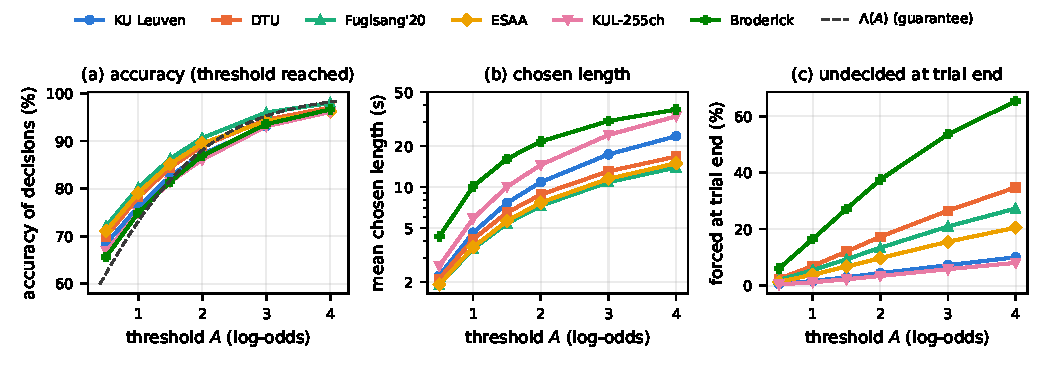
\includegraphics[width=\textwidth]{figures/conf_threshold.pdf}
\caption{Effect of the threshold $A$. (a) Accuracy of the decisions that reached the
threshold, against the guarantee $\Lambda(A)$ (dashed). (b) Mean chosen length. (c) Share of
decisions cut by the end of a trial.}\label{fig:conf_threshold}
\end{figure*}
\begin{figure*}[h]\centering
{\small (a) distribution of the chosen length}\\[2pt]
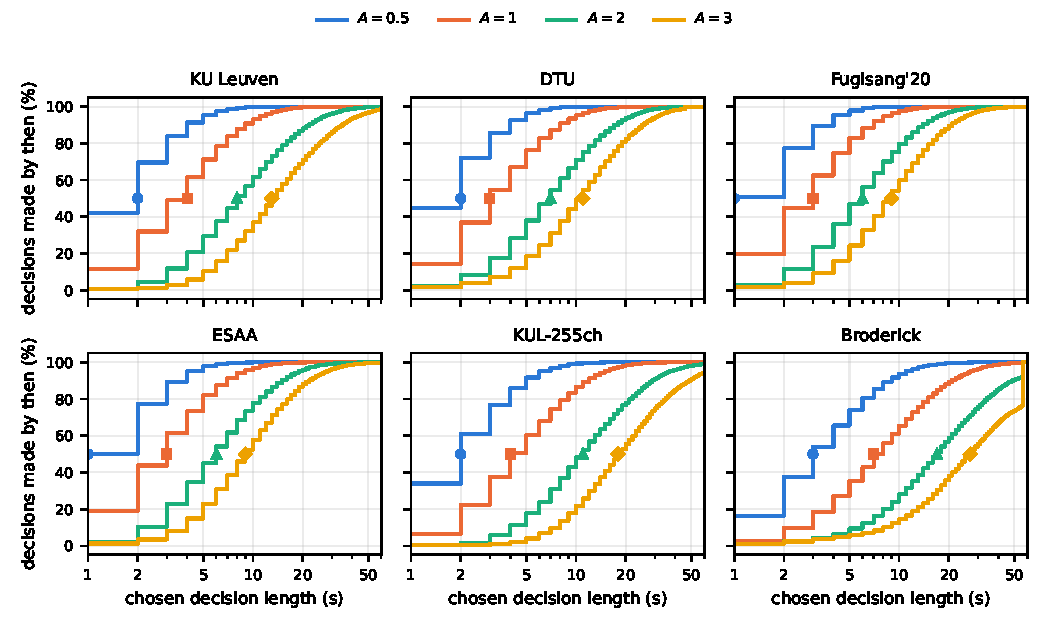
\includegraphics[width=0.85\textwidth]{figures/conf_lengths.pdf}\\[6pt]
{\small (b) accuracy by chosen length}\\[2pt]
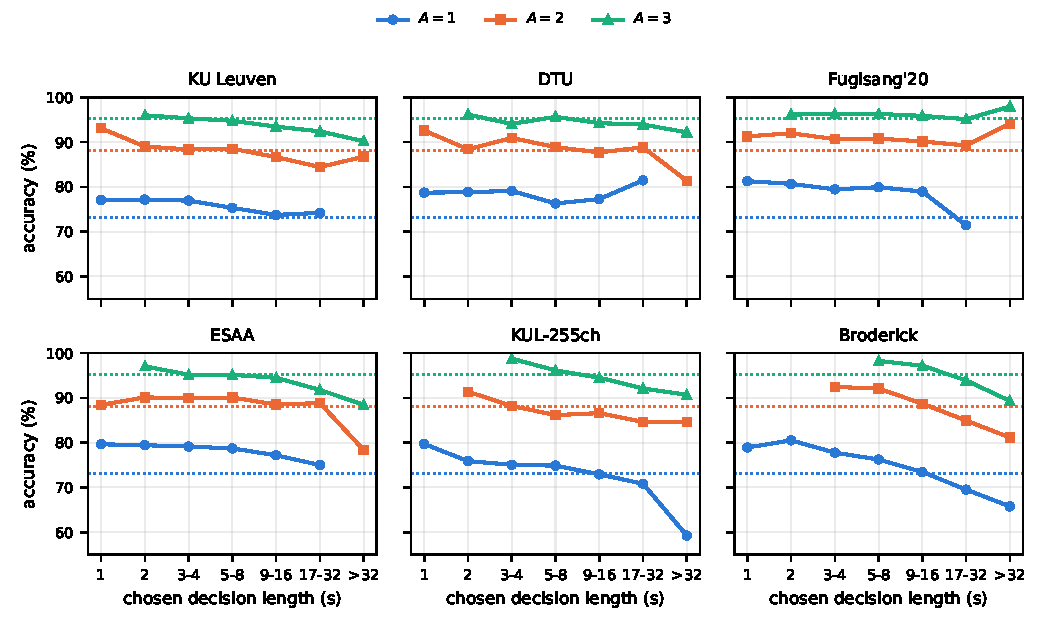
\includegraphics[width=0.85\textwidth]{figures/conf_acc_by_length.pdf}
\caption{The chosen decision length. (a) Share of decisions taken within a given number of
seconds, for four thresholds; markers: medians. (b) Accuracy of the decisions that reached the
threshold, grouped by the length they used, for $A=1,2,3$. Dotted: $\Lambda(A)$, the accuracy
Prop.~\ref{prop:stop} guarantees for every length. Bins with fewer than 20 decisions are
omitted.}\label{fig:conf_len}
\end{figure*}

\subsection{Overlapping windows}\label{app:conf:overlap}
Table~\ref{tab:conf_overlap} and Fig.~\ref{fig:conf_overlap} repeat the analysis with 1-s
windows every 0.5\,s and 0.25\,s (CoupleFlow, seed 0). The data follow
Prop.~\ref{prop:overlap} closely. The log-odds of windows $jh$ apart correlate as
$1-jh/w$ (KU Leuven, hop 0.25\,s: \confOvCorOne, \confOvCorTwo, \confOvCorThree{} at
$j=1,2,3$; prediction 0.75, 0.5, 0.25), fixed-length accuracy changes by at most
\confOvFixedMax{} points, and the summed log-odds are over-confident (5-s ECE up to
\confOvEceRawMax) until scaled by $h/w$ (ECE $\le$\,\confOvEceCorrMax). The corrected
sequential rule gains \confOvSeqMin--\confOvSeqMax{} points over the non-overlapping one at
the same mean time, the small effect of checking the threshold more often. One detail
matters: after a decision the rule must restart at the first window that shares no data with
that decision. Restarting at the adjacent window re-uses the window that crossed the
threshold and inflates accuracy at $A{=}2$ by \confOvAdjMin--\confOvAdjMax{} points without any
new evidence.
\begin{figure*}[h]\centering
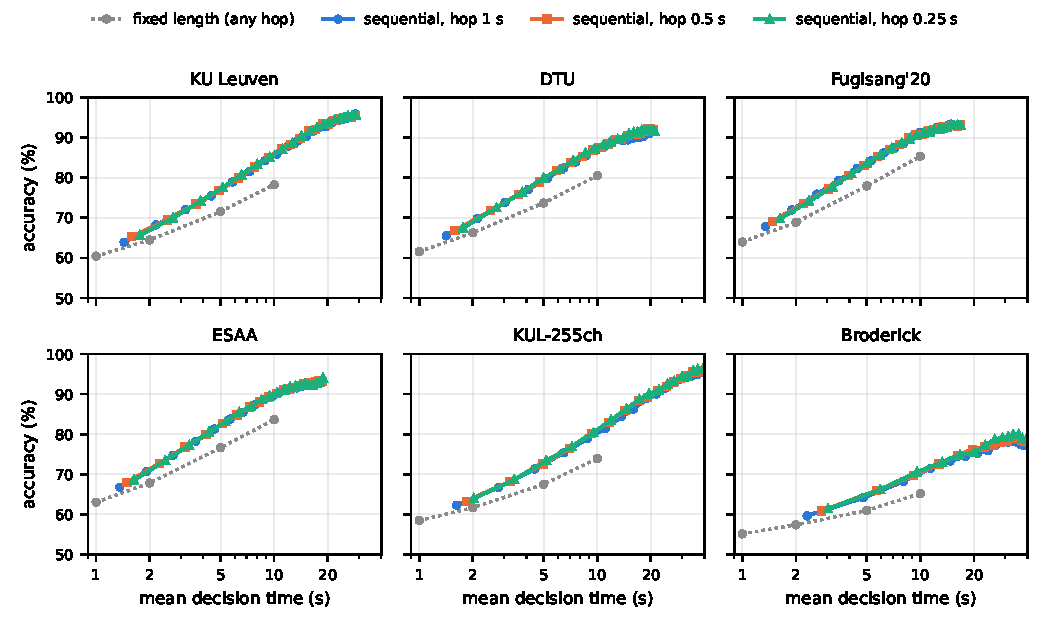
\includegraphics[width=0.95\textwidth]{figures/conf_overlap.pdf}
\caption{Overlapping 1-s windows (CoupleFlow, seed 0, test folds): the sequential rule on
$h/w$-scaled log-odds with hop $h=1$, 0.5 and 0.25\,s, restarting after each decision at the
first window disjoint from it, and fixed-length decisions (nearly identical for every hop; the hop-1\,s curve is shown).}\label{fig:conf_overlap}
\end{figure*}
\begin{table*}[h]\centering\small
\caption{Overlapping 1-s windows (CoupleFlow, seed 0). Fixed 5\,s: accuracy of the summed
log-odds of the windows inside each 5-s stretch. ECE of those sums without (raw) and with the
$h/w$ correction. Seq.: corrected sequential rule at $A{=}2$, accuracy (\%) / mean time
(s).}\label{tab:conf_overlap}
\resizebox{\textwidth}{!}{\begin{tabular}{lccccccccc}\toprule
& \multicolumn{3}{c}{hop 1\,s} & \multicolumn{3}{c}{hop 0.5\,s} & \multicolumn{3}{c}{hop 0.25\,s} \\
\cmidrule(lr){2-4}\cmidrule(lr){5-7}\cmidrule(lr){8-10}
Dataset & fixed 5\,s & ECE raw/corr. & seq.\ $A{=}2$ & fixed 5\,s & ECE raw/corr. & seq.\ $A{=}2$ & fixed 5\,s & ECE raw/corr. & seq.\ $A{=}2$ \\\midrule
KU Leuven & 71.5 & 0.04/0.04 & 85.9 / 10.4 & 71.8 & 0.12/0.02 & 87.1 / 11.0 (+0.5) & 71.6 & 0.19/0.02 & 87.1 / 11.1 (+0.4) \\
DTU & 73.7 & 0.02/0.02 & 85.5 / 8.7 & 74.2 & 0.10/0.01 & 86.9 / 9.4 (+0.6) & 74.3 & 0.17/0.01 & 87.2 / 9.7 (+0.6) \\
Fuglsang'20 & 77.9 & 0.01/0.01 & 87.5 / 7.2 & 77.3 & 0.10/0.01 & 88.2 / 7.7 (+0.2) & 77.2 & 0.15/0.01 & 88.6 / 7.9 (+0.3) \\
ESAA & 76.6 & 0.02/0.02 & 87.3 / 7.8 & 76.6 & 0.10/0.01 & 88.0 / 8.3 (+0.1) & 76.6 & 0.16/0.01 & 88.7 / 8.5 (+0.4) \\
KUL-255ch & 67.5 & 0.03/0.03 & 86.3 / 16.0 & 68.0 & 0.11/0.02 & 88.5 / 17.2 (+1.2) & 67.6 & 0.20/0.01 & 88.7 / 17.3 (+1.3) \\
Broderick & 61.0 & 0.03/0.03 & 75.9 / 24.0 & 61.1 & 0.10/0.02 & 77.2 / 25.7 (+0.3) & 60.8 & 0.19/0.02 & 78.7 / 26.2 (+1.6) \\
\bottomrule\end{tabular}
}
\end{table*}

\subsection{Training-window length}\label{app:conf:trainlen}
% Training-window ablation; numbers from tables/numbers_conf.tex.
The paper's models are trained on 5-s crops and applied at every test window. We retrained
CoupleFlow with 1-, 2- and 10-s crops, and with a crop length redrawn from $\{1,2,5,10\}$\,s
at every epoch (``mixed''), keeping everything else fixed: the same folds, seeds, losses,
epochs, and model selection on 5-s validation windows (Fig.~\ref{fig:conf_trainlen},
Table~\ref{tab:conf_trainlen}). Differences below are against the paper's 5-s training, mean of
3 seeds, over all 8 datasets.

\emph{Short crops help short windows.} Training on 1-s crops raises 1-s accuracy by
\confTlOneOneSMin{} to \confTlOneOneSMax{} points ($n=$\,\confTlOneOneSN{} datasets), but
changes 5-s accuracy by \confTlOneFiveSMin{} to \confTlOneFiveSMax{} and 30-s accuracy by
\confTlOneThirtySMin{} to \confTlOneThirtySMax. \emph{Long crops help nothing}: 10-s training
changes 1-s accuracy by \confTlTenOneSMin{} to \confTlTenOneSMax{} and 5-s accuracy by
\confTlTenFiveSMin{} to \confTlTenFiveSMax{} points.

\emph{Mixed crops are best overall.} Redrawing the crop length raises 1-s accuracy on every dataset
(\confTlMixOneSMin{} to \confTlMixOneSMax{} points, $n=$\,\confTlMixOneSN) and lowers neither
5-s accuracy (\confTlMixFiveSMin{} to \confTlMixFiveSMax) nor 30-s accuracy
(\confTlMixThirtySMin{} to \confTlMixThirtySMax) by more than 0.1 points. In the terms of Prop.~\ref{prop:gauss} it raises
the information rate of the 1-s evidence: $\kappa$ of the summed 1-s log-odds grows by a factor
\confTlMixKapMin--\confTlMixKapMax, and the sequential rule at $A{=}2$ needs
\confTlMixTimeMin--\confTlMixTimeMax{} of the time (\confTlOneTimeMin--\confTlOneTimeMax{}
for 1-s training). A plausible reading, which we have not tested further: a model that only sees long crops learns a coupling that is reliable when
averaged over many seconds but noisy within one; short crops force every second to carry
evidence, and mixing lengths keeps the long-window accuracy. The paper's main results use
5-s training throughout; mixed-length training is a free improvement for any window.

\begin{figure*}[h]\centering
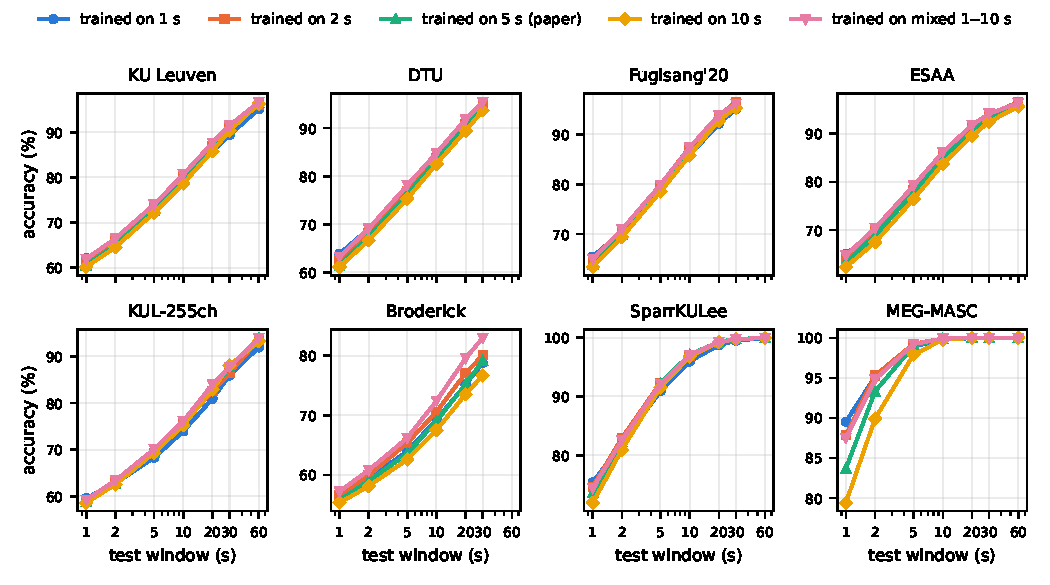
\includegraphics[width=0.95\textwidth]{figures/conf_trainlen.pdf}
\caption{Test accuracy against test window for CoupleFlow trained on 1-, 2-, 5- (paper),
10-s crops or a length redrawn from $\{1,2,5,10\}$\,s every epoch; everything else as in the
paper (selection on 5-s validation windows). Mean of 3 seeds, test folds; competing talker for
two-talker sets, match--mismatch for SparrKULee and MEG-MASC.}\label{fig:conf_trainlen}
\end{figure*}
\begin{table*}[h]\centering\small
\caption{Training-window ablation: accuracy (\%, mean$\pm$s.d.\ over 3 seeds) at 1-, 5- and
30-s test windows, $\kappa$ of the summed 1-s log-odds, and the sequential rule at $A{=}2$
(two-talker sets).}\label{tab:conf_trainlen}
\resizebox{0.8\textwidth}{!}{\begin{tabular}{llccccc}\toprule
Dataset & training window & 1\,s & 5\,s & 30\,s & $\kappa$ (1-s sums) & seq.\ $A{=}2$: acc.\ / time \\\midrule
KU Leuven & 1 s & 62.1{\scriptsize$\pm$0.3} & 72.9{\scriptsize$\pm$0.6} & 89.4{\scriptsize$\pm$0.2} & 0.251 & 85.4 / 8.1 \\
 & 2 s & 61.5{\scriptsize$\pm$0.2} & 73.4{\scriptsize$\pm$0.6} & 91.2{\scriptsize$\pm$0.3} & 0.252 & 86.2 / 9.3 \\
 & 5 s (paper) & 60.5{\scriptsize$\pm$0.1} & 72.7{\scriptsize$\pm$0.2} & 90.5{\scriptsize$\pm$0.4} & 0.240 & 86.6 / 10.9 \\
 & 10 s & 60.2{\scriptsize$\pm$0.1} & 72.2{\scriptsize$\pm$0.6} & 90.3{\scriptsize$\pm$0.5} & 0.231 & 86.4 / 11.8 \\
 & mixed 1--10 s & 62.0{\scriptsize$\pm$0.3} & 74.0{\scriptsize$\pm$0.4} & 91.5{\scriptsize$\pm$0.6} & 0.259 & 86.5 / 8.7 \\
\midrule
DTU & 1 s & 63.9{\scriptsize$\pm$0.0} & 77.1{\scriptsize$\pm$0.3} & 94.3{\scriptsize$\pm$0.2} & 0.308 & 86.9 / 6.6 \\
 & 2 s & 62.5{\scriptsize$\pm$0.1} & 76.9{\scriptsize$\pm$0.5} & 94.8{\scriptsize$\pm$0.8} & 0.287 & 86.2 / 7.7 \\
 & 5 s (paper) & 61.4{\scriptsize$\pm$0.3} & 76.2{\scriptsize$\pm$0.6} & 94.5{\scriptsize$\pm$0.8} & 0.267 & 85.5 / 8.8 \\
 & 10 s & 61.1{\scriptsize$\pm$0.2} & 75.3{\scriptsize$\pm$0.3} & 93.7{\scriptsize$\pm$0.8} & 0.259 & 85.3 / 9.8 \\
 & mixed 1--10 s & 63.2{\scriptsize$\pm$0.1} & 78.1{\scriptsize$\pm$0.2} & 95.4{\scriptsize$\pm$0.2} & 0.304 & 86.5 / 6.9 \\
\midrule
Fuglsang'20 & 1 s & 65.4{\scriptsize$\pm$0.1} & 78.8{\scriptsize$\pm$0.2} & 95.1{\scriptsize$\pm$0.5} & 0.331 & 87.5 / 6.0 \\
 & 2 s & 64.5{\scriptsize$\pm$0.3} & 79.9{\scriptsize$\pm$0.4} & 96.5{\scriptsize$\pm$0.2} & 0.330 & 87.5 / 6.6 \\
 & 5 s (paper) & 63.8{\scriptsize$\pm$0.3} & 79.6{\scriptsize$\pm$0.8} & 95.9{\scriptsize$\pm$1.3} & 0.318 & 87.5 / 7.3 \\
 & 10 s & 63.4{\scriptsize$\pm$0.2} & 78.5{\scriptsize$\pm$0.1} & 95.4{\scriptsize$\pm$0.3} & 0.312 & 87.7 / 7.8 \\
 & mixed 1--10 s & 64.9{\scriptsize$\pm$0.2} & 79.9{\scriptsize$\pm$0.4} & 96.2{\scriptsize$\pm$0.2} & 0.339 & 87.9 / 6.4 \\
\midrule
ESAA & 1 s & 65.1{\scriptsize$\pm$0.1} & 78.3{\scriptsize$\pm$0.4} & 94.2{\scriptsize$\pm$0.6} & 0.316 & 87.2 / 6.0 \\
 & 2 s & 64.0{\scriptsize$\pm$0.3} & 78.4{\scriptsize$\pm$0.4} & 93.9{\scriptsize$\pm$0.3} & 0.309 & 87.6 / 6.9 \\
 & 5 s (paper) & 63.2{\scriptsize$\pm$0.3} & 77.9{\scriptsize$\pm$0.3} & 93.4{\scriptsize$\pm$0.5} & 0.292 & 87.3 / 7.7 \\
 & 10 s & 62.3{\scriptsize$\pm$0.4} & 76.4{\scriptsize$\pm$0.1} & 92.4{\scriptsize$\pm$0.3} & 0.275 & 87.0 / 9.0 \\
 & mixed 1--10 s & 64.7{\scriptsize$\pm$0.1} & 79.2{\scriptsize$\pm$0.1} & 94.2{\scriptsize$\pm$0.4} & 0.310 & 87.4 / 6.4 \\
\midrule
KUL-255ch & 1 s & 59.6{\scriptsize$\pm$0.3} & 68.3{\scriptsize$\pm$0.2} & 85.9{\scriptsize$\pm$0.4} & 0.200 & 84.2 / 12.3 \\
 & 2 s & 59.0{\scriptsize$\pm$0.3} & 69.3{\scriptsize$\pm$0.6} & 86.4{\scriptsize$\pm$0.6} & 0.208 & 84.7 / 13.2 \\
 & 5 s (paper) & 58.9{\scriptsize$\pm$0.3} & 69.4{\scriptsize$\pm$0.4} & 87.7{\scriptsize$\pm$0.9} & 0.203 & 86.0 / 14.7 \\
 & 10 s & 58.6{\scriptsize$\pm$0.3} & 69.4{\scriptsize$\pm$0.4} & 88.1{\scriptsize$\pm$1.2} & 0.201 & 85.1 / 14.4 \\
 & mixed 1--10 s & 59.3{\scriptsize$\pm$0.2} & 70.1{\scriptsize$\pm$0.3} & 87.7{\scriptsize$\pm$0.6} & 0.214 & 85.5 / 12.7 \\
\midrule
Broderick & 1 s & 56.8{\scriptsize$\pm$0.3} & 64.0{\scriptsize$\pm$0.5} & 78.8{\scriptsize$\pm$0.3} & 0.149 & 79.4 / 17.6 \\
 & 2 s & 56.6{\scriptsize$\pm$0.5} & 65.4{\scriptsize$\pm$1.0} & 80.1{\scriptsize$\pm$2.6} & 0.146 & 80.0 / 18.9 \\
 & 5 s (paper) & 55.8{\scriptsize$\pm$0.7} & 63.6{\scriptsize$\pm$1.8} & 79.2{\scriptsize$\pm$2.6} & 0.131 & 77.7 / 22.0 \\
 & 10 s & 55.3{\scriptsize$\pm$0.9} & 62.6{\scriptsize$\pm$2.1} & 76.7{\scriptsize$\pm$3.5} & 0.119 & 76.6 / 24.1 \\
 & mixed 1--10 s & 57.2{\scriptsize$\pm$0.4} & 66.2{\scriptsize$\pm$0.6} & 83.0{\scriptsize$\pm$1.0} & 0.160 & 81.0 / 16.7 \\
\midrule
SparrKULee & 1 s & 75.4{\scriptsize$\pm$0.1} & 90.9{\scriptsize$\pm$0.1} & 99.5{\scriptsize$\pm$0.0} & -- & -- \\
 & 2 s & 74.6{\scriptsize$\pm$0.1} & 92.3{\scriptsize$\pm$0.1} & 99.7{\scriptsize$\pm$0.0} & -- & -- \\
 & 5 s (paper) & 73.5{\scriptsize$\pm$0.0} & 92.2{\scriptsize$\pm$0.0} & 99.7{\scriptsize$\pm$0.1} & -- & -- \\
 & 10 s & 71.9{\scriptsize$\pm$0.0} & 91.5{\scriptsize$\pm$0.1} & 99.7{\scriptsize$\pm$0.0} & -- & -- \\
 & mixed 1--10 s & 74.4{\scriptsize$\pm$0.2} & 92.2{\scriptsize$\pm$0.0} & 99.7{\scriptsize$\pm$0.0} & -- & -- \\
\midrule
MEG-MASC & 1 s & 89.5{\scriptsize$\pm$0.2} & 98.9{\scriptsize$\pm$0.1} & 100.0{\scriptsize$\pm$0.0} & -- & -- \\
 & 2 s & 87.8{\scriptsize$\pm$0.3} & 99.3{\scriptsize$\pm$0.1} & 100.0{\scriptsize$\pm$0.0} & -- & -- \\
 & 5 s (paper) & 83.7{\scriptsize$\pm$0.4} & 99.0{\scriptsize$\pm$0.1} & 100.0{\scriptsize$\pm$0.0} & -- & -- \\
 & 10 s & 79.4{\scriptsize$\pm$0.5} & 97.9{\scriptsize$\pm$0.1} & 100.0{\scriptsize$\pm$0.0} & -- & -- \\
 & mixed 1--10 s & 87.5{\scriptsize$\pm$0.7} & 99.2{\scriptsize$\pm$0.1} & 100.0{\scriptsize$\pm$0.0} & -- & -- \\
\bottomrule\end{tabular}
}
\end{table*}
